\section{Object Oriented Design}
In this section we'll provide a brief illustration for OOD in our final project \textbf{Make It On Time}. Although we won't go through the detailed design and responsibility for each class, we do provide a simplified version of class diagrams, which demonstrate the relations between our classes.\\
There are three major division of classes in our design: 
\begin{enumerate}
\item The \textbf{model} of the world, which includes all sorts of objects inside the game world and encapsulates their relations.
\item The \textbf{controller}, which is the interface between player input and the game world.
\item The \textbf{View}, which is responsible for displaying the world to  the player.
\end{enumerate}
\begin{figure}[h!]

\begin{subfigure}{\textwidth}
\centering
  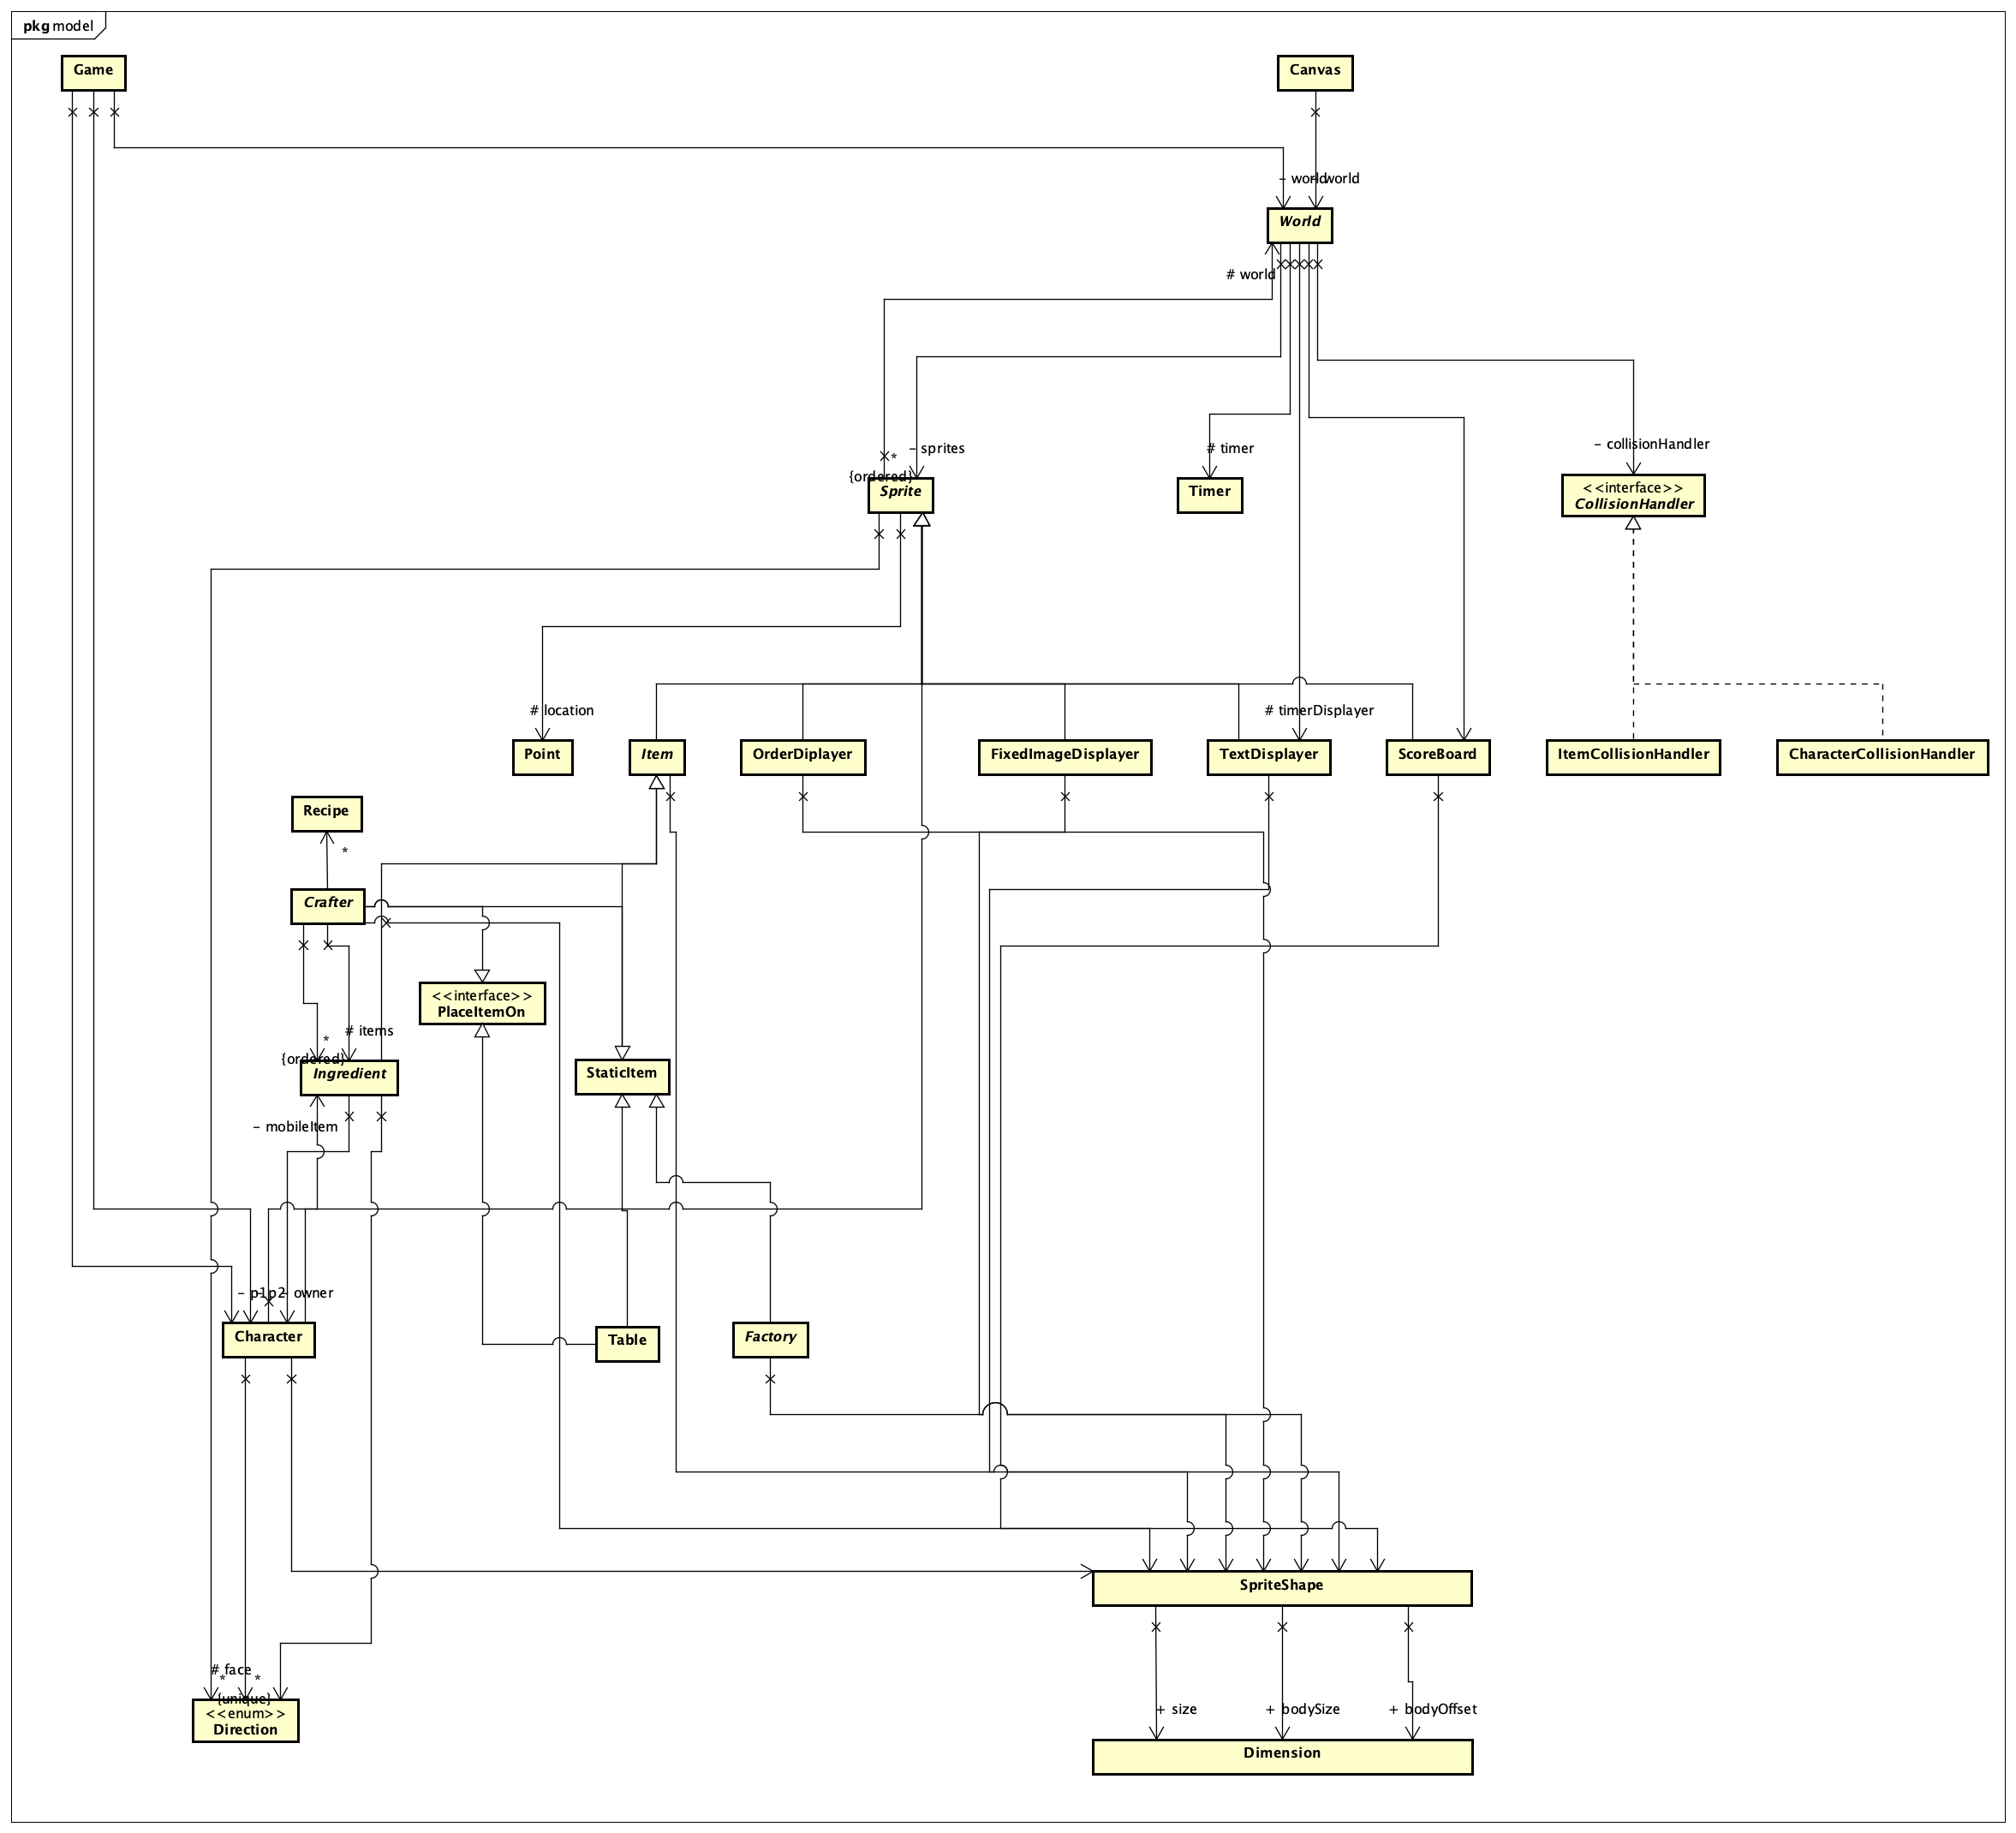
\includegraphics[width=.9\linewidth]{Model_Class_Diagram}  
  \caption{A simplified class diagram of \textbf{World}.}
  \label{fig}
\end{subfigure}

\begin{subfigure}{.5\textwidth}
\centering
  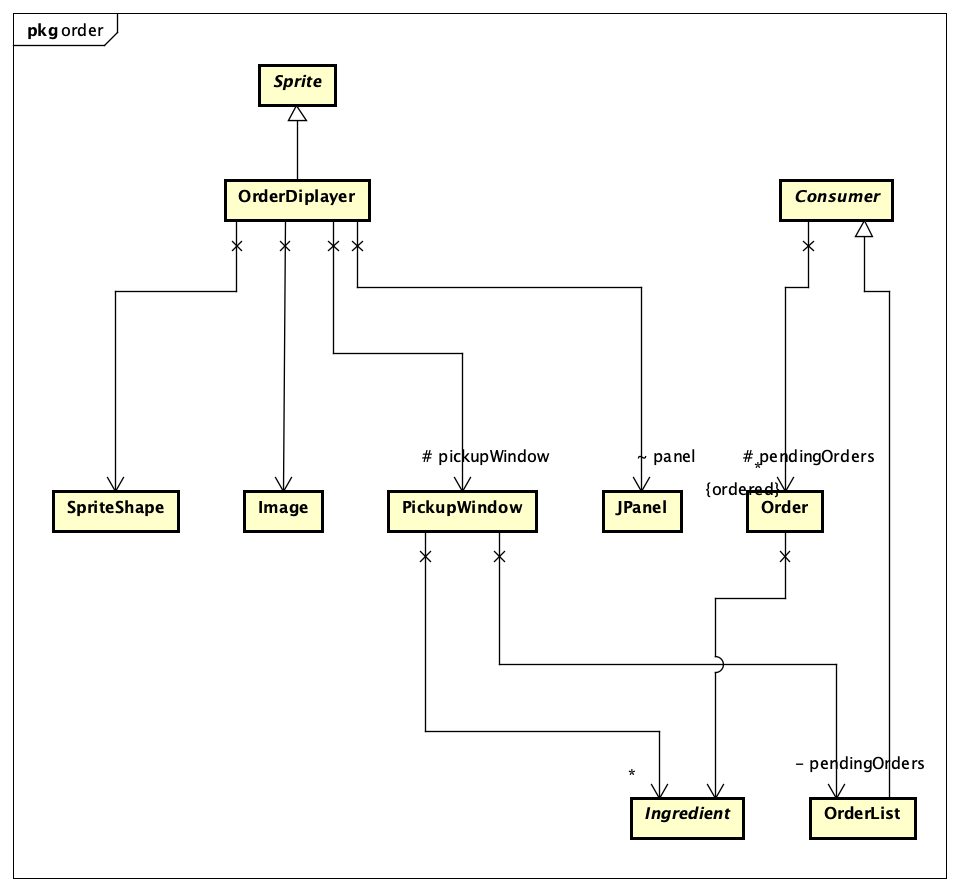
\includegraphics[width=.9\linewidth]{Order_Class_Diagram}  
  \caption{A simplified class diagram of \textbf{OrderList}.}
  \label{fig:sub-first}
\end{subfigure}
\begin{subfigure}{.5\textwidth}
  \centering
  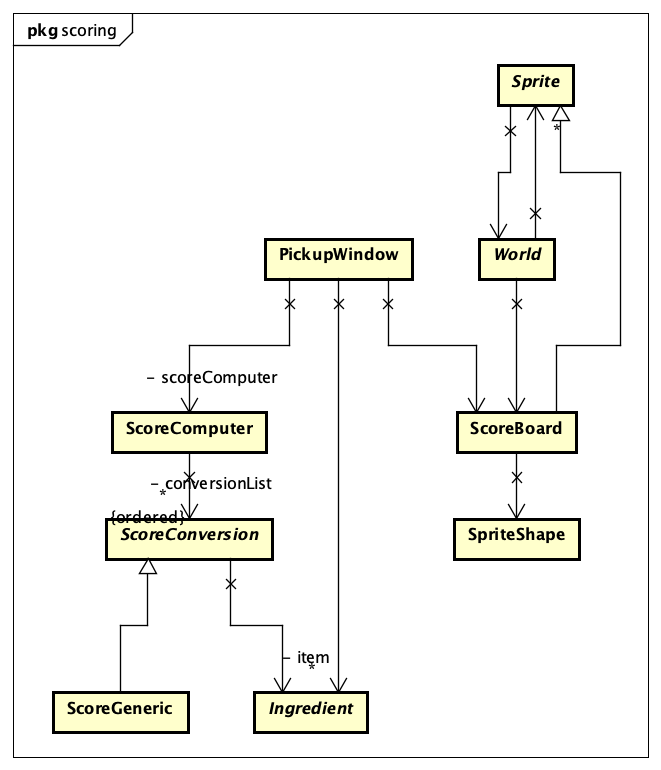
\includegraphics[width=.9\linewidth]{Score_Class_Diagram}  
  \caption{A simplified class diagram of \textbf{Scoreboard}.}
  \label{fig:sub-second}
\end{subfigure}
\caption{Class diagrams of the game model in this project.}
\end{figure}
\subsection{Model}
The model of our game world is implemented in the class file \textbf{World}, which contains the following attributes. as shown in \textit{Figure 1-(a)}.
\begin{enumerate}
\item \textit{Sprite}, a collection of the \textbf{Sprite} residing in our game world, they can further be classified into several classes
\begin{enumerate}
\item \textbf{Character}, which can be controlled by players and is able to interact with other items, e.g. picking and releasing \textbf{MobileItem}, and collision with \textbf{StaticItem}.
\item \textbf{Item}, which includes all sprites other than player in our game, divided into
\begin{enumerate}
\item \textbf{MobileItem}, or equivalently \textbf{Ingredient} in our design, which can be picked up and moved with \textbf{Character}. Also they can interact with \textbf{StaticItem} to be discarded and crafted into a new \textbf{Ingredient}.
\item \textbf{StaticItem}, which isn't mobile but may be equipped with different function, allowing them to interact with \textbf{MobileItem} and \textbf{Character}. (See the following subsection for details)
\end{enumerate}

\end{enumerate}
\item \textbf{OrderDisplayer} is a special sprite, which shows the incoming order, requiring character to deliver them.
\item \textbf{Scoreboard} is also a special sprite, demonstrating the score player had gotten via controlling \textbf{Character} to complete the orders.\\
The simplified class diagram of \textbf{OrderDisplayer} and \textbf{Scoreboard} are shown in \textit{Figure 1-(b), (c)}, and worth noting is that they can interact with \textbf{Ingredient} (or completed order the player make) via a static item \textbf{PickUpWindow} is our design.
\item \textbf{Timer}, which counts down the game time.
\item \textbf{TextDisplayer} and \textbf{FixedImageDisplayer}. As the name suggested, these items can display text and images in the \textbf{World} as background.
\item \textbf{CollisionHandler}, which is responsible to handle the overlap the rigid body between sprites.
\end{enumerate}
\subsubsection{Detail about Item Relations}
Several type of static items are implemented with some properties allowing them to interact with mobile item, or \textbf{Ingredient}. These includes,
\begin{enumerate}
\item \textbf{Factory}, an abstract class, which encapsulate the function of limitlessly produce ingredient.
\item \textbf{Crafter}, an abstract class, which encapsulate the function of transforming ingredient(s) into new ingredient. Inside the \textbf{Crafter} are several \textbf{Recipe} attributes enclosing the transform formula.
\item \textbf{PlaceItemOn}, an interface which allows ingredient(s) to be  released on this item.
\end{enumerate}
\begin{figure}[h!]
\begin{subfigure}{.5\textwidth}
\centering
  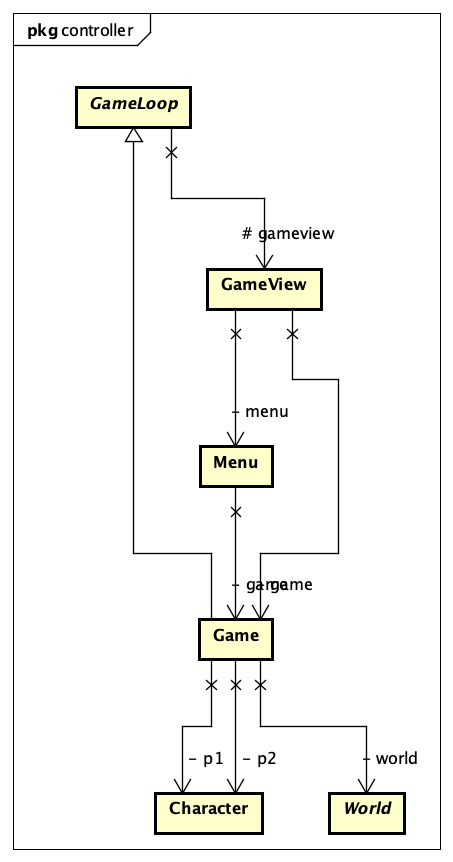
\includegraphics[width=.9\linewidth]{Controller_Class_Diagram}  
  \caption{A simplified class diagram of game controller in this project.}
  \label{fig:sub-first}
\end{subfigure}
\begin{subfigure}{.5\textwidth}
  \centering
  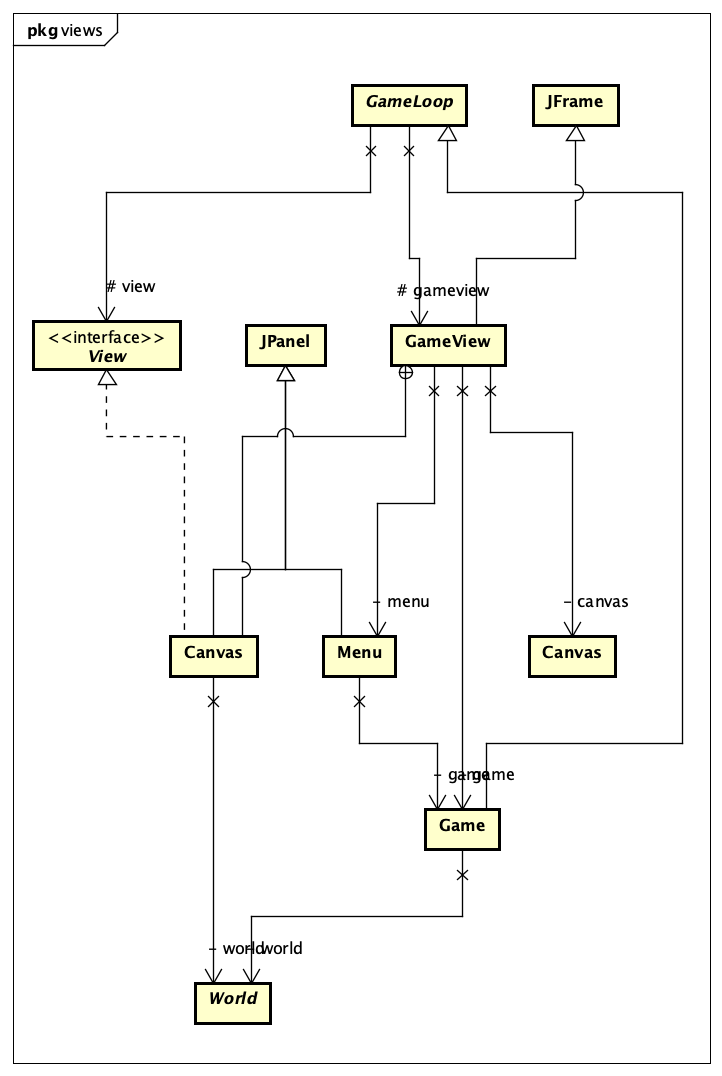
\includegraphics[width=.9\linewidth]{View_Class_Diagram}  
  \caption{A simplified class diagram of game view in the project.}
  \label{fig:sub-second}
\end{subfigure}
\caption{Class diagrams of the game control and view in this project.}
\end{figure}

\subsection{Controller}
As shown in \textit{Figure 2-(a)}, class \textbf{Game} implementing \textbf{GameLoop} operates the game flow, and \textbf{GameView} allows player to interact with \textbf{Game} and \textbf{Menu}, which in terms alters the \textbf{Character} and \textbf{World}.

\subsection{View}
As shown in \textit{Figure 2-(b)}, class \textbf{GameView} utilizes \textbf{Canvas} to render the world and the action of the character in it.
\newpage